\documentclass{article}
\usepackage{tikz}
\usetikzlibrary{positioning,calc}
\begin{document}
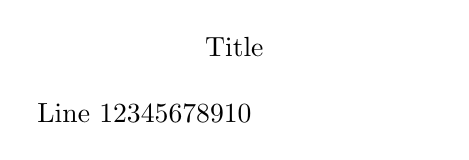
\begin{tikzpicture}
\node (A) at (0, 3.5) {Title};
\node[below=3.5mm of A] (B) {\parbox{5cm}{Line 1\Line 2\Line 3\Line 4\Line 5\Line 6\Line 7\Line 8\Line 9\Line 10}};
\path (B.north west); \pgfgetlastxy{\macrox}{\macroy} \typeout{B.north west: \macrox, \macroy}
\path (B.west); \pgfgetlastxy{\macrox}{\macroy} \typeout{B.west: \macrox, \macroy}
\path (B.south west); \pgfgetlastxy{\macrox}{\macroy} \typeout{B.south west: \macrox, \macroy}
\end{tikzpicture}
\end{document}
